%%%%%%
%
% PROJECT 4 - ASTRONOMERS USE PARABOLIC MIRRORS
%
% filename: astronomers_use_parabolic_mirrors.tex
% last modified: 2014-7-16
%
%%%%%%%
%
%
%%%%%%%

\documentclass
[justified,nohyper]
{tufte-handout}

\usepackage{amsmath}
\usepackage{amsthm}

\usepackage{booktabs}
\usepackage{graphicx}
\usepackage{kmath,kerkis} % The order of the packages matters; kmath changes the default text font
\usepackage[T1]{fontenc}


\newtheoremstyle{mydef}
{\topsep}{\topsep}%
{}{}%
{\bfseries}{}
{\newline}
{%
  \rule{\textwidth}{0.4pt}\\*%
  \thmname{#1}~\thmnumber{#2}\thmnote{\ -\ #3}.\\*[-1.5ex]%
  \rule{\textwidth}{0.4pt}}%

\theoremstyle{mydef}
\newtheorem{definition}{Definition}

\begin{document}
\section{Advanced Calculus Project 4: Astronomers Use Parabolic Mirrors}

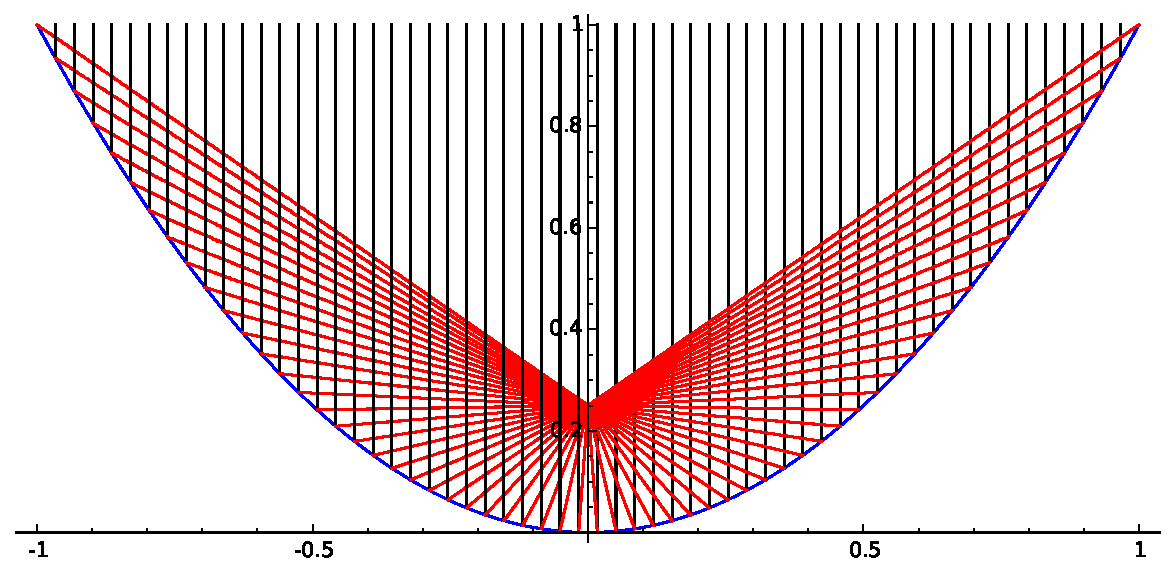
\includegraphics[width=10cm]{parabolic.pdf}

\newthought{The star nearest our sun} is Alpha Centauri, which is about 4 light years from earth. Alpha Centauri is so far away that when its light reaches earth, it is traveling in essentially parallel rays. To observe distant stars, astronomers use mirrors shaped like paraboloids, which are parabolas rotated about their axes. The reason they use a paraboloidal mirror is that it focuses all the light to a single point, the ``focus.'' (This point is the image of the star in the paraboloidal mirror.) In this project you will demonstrate the focusing property of parabolas.

Suppose our mirror is shaped like the parabola $y=kx^2$, where $k$ is any positive constant. Find the coordinates of its focus and the equation of its directrix in terms of $k$.

The following guided questions are meant to stimulate your thinking about what's going on. Your first step should be to sketch answers to these questions on notebook paper and let that thinking guide the development of your report. It is important to start with paper because ideas flow easily when you have a pencil in hand. However, as these ideas begin to develop, you will want to make the transition into SageCloudMath and start constructing real graphs.

As always, your report should contain an abstract, procedure, and conclusion. Your report should flow from beginning to end and represent a smooth transition between ideas to arrive at your conclusion: that astronomers use parabolic mirrors to look at stars.

Find the equation of the line tangent to the parabola at a point $(x_0,y_0)$ on the parabola. Then find the $y$-intercept of the tangent line.

Consider the triangle formed by a point $(x_0,y_0)$ on the parabola, the $y$-intercept of the tangent line at this point, and the focus -- remember that you found the focus in terms of $k$ at beginning of this project. Plot a picture of this triangle. Prove the triangle is isosceles.

Suppose an incoming light ray strikes a parabola at a point $(x_0,y_0)$. If the light ray makes an angle $\gamma$ with respect to the tangent line, then it is reflected at an equal angle to the tangent line. This result from physics is known by the phrase ``the angle of incidence equals the angle of reflection.'' Using this fact, argue that incoming light rays parallel to the axis of the parabola are all reflected to the focus, independent of the point of incidence. This fact is demonstrated by the picture at the beginning of this project description. You must duplicate this graph in SageCloudMath to demonstrate that you know what's going on. The conclusion from this graph is that a parabolic mirror focuses incoming light rays parallel to the axis to a point.

The path followed by a ray of light from the star to the focus of the mirror has another special property. Draw a chord of the parabola that is above the focus and parallel to the directrix. Consider a ray of light parallel to the $y$-axis as it crosses the chord, hits the parabola and is reflected to the focus. Let $d_1$ be the distance from the chord to the point of incidence $(x_0,y_0)$ on the parabola and let $d_2$ be the distance from $(x_0,y_0)$ to the focus. Show that the sum of the distances $d_1+d_2$ is constant, independent of the particular point of incidence. Since light travels at constant velocity, explain why this special property is very relevant for astronomers.

Extend your argument from the parabolic cross section to the entire paraboloidal mirror, obtained by rotating this cross section about the $y$-axis. Thus, prove that all incident rays parallel to the axis of such a mirror focus to a point. Also prove that light traveling along different rays to the focus from a chord perpendicular to the axis will have travelled the same distance, even though these rays were reflected from different points of incidence on the mirror. Thus all of the light waves will arrive in phase, and so will interfere constructively to produce a nice bright spot as the image of the star.

\end{document}